\section{Empirical Case Studies}
\label{sec:case_studies}

The empirical evidence serves two purposes: SS6 illustrates the
reliability quantities on MAST-derived framework summaries, while SS9
uses a strict held-out split to test whether \textsc{TraceToChain}
recovers the RDC and success-time distribution on unseen traces.

\subsection{MAST Benchmark Formulation}
\label{sec:mast}

SS6 uses transition matrices derived from public MAST summaries for
seven frameworks, applies the fitted-chain quantities, and ranks
frameworks by $R_\infty$. The exercise is illustrative: it does not
claim that raw MAST traces are Markov, but it shows what the reliability
vocabulary reports once a chain is available. Asymptotic reliability
spans $R_\infty\in[0.058,0.450]$: it is highest for
toolformer~\cite{schick2023toolformer} and lowest
($\le\!0.07$) for react~\cite{yao2023react}, cot\_agent, and
reflexion~\cite{shinn2023reflexion}, over
$m\in[5,12]$ states with $\rho(Q)\in[0.37,0.66]$ and $\delta{=}0.01$
horizons of $3$--$9$ steps. The full table and the corresponding decay
curves are in the artifact.

%% [REDUCTION] The illustrative SS6 table is suppressed for the 12-page body;
%% its range is quoted inline above and the full table is in the artifact.
\iffalse
\begin{table}[!t]
\centering
\caption{Closed-Form Reliability of MAST Frameworks.}
\label{tab:mast}
\begin{tabular}{lrrrr}
\toprule
\textbf{Framework} & \textbf{$R_\infty$} & \textbf{$\rho(Q)$} & \textbf{Horizon ($\delta=0.01$)} & \textbf{$m$} \\
\midrule
\thighlight
toolformer~\cite{schick2023toolformer}  & 0.4497 & 0.442 &  5 & 10 \\
\tstriped
autogpt~\cite{wang2024agentsurvey}     & 0.3866 & 0.370 &  4 &  5 \\
agentbench~\cite{agentbench2024}  & 0.3262 & 0.654 &  9 & 10 \\
\tstriped
babyagi~\cite{wang2024agentsurvey}     & 0.2853 & 0.656 &  8 & 12 \\
reflexion~\cite{shinn2023reflexion}   & 0.0695 & 0.636 &  5 & 12 \\
\tstriped
cot\_agent~\cite{wang2024agentsurvey}  & 0.0684 & 0.526 &  3 & 10 \\
react~\cite{yao2023react}       & 0.0581 & 0.509 &  3 &  9 \\
\bottomrule
\end{tabular}
\end{table}
\fi


\subsection{SS9: Held-Out Empirical Validation}
\label{sec:ss9}

SS7(C) is an in-sample self-consistency check; SS9 instead evaluates
controlled held-out recovery with a strict fit/test protocol. The test
set is not used to choose features, clusters, transition estimates, or
tuning, so the reported KS and RDC errors measure held-out recovery
rather than reuse of the training corpus.

\paragraph{Protocol.}
For each of the 7 MAST-style frameworks we generate $n=400$
trajectories from a ground-truth absorbing chain whose transient
structure mimics the MAST taxonomy and emits noisy one-hot features
(Gaussian noise $\sigma=0.08$ and $\approx\!5\%$ censored traces). The
corpus is split \emph{before} featurization into
$n_{\mathrm{fit}}=200$ and $n_{\mathrm{test}}=200$. We run
\textsc{TraceToChain} on the fit half only.

Table~\ref{tab:heldout-ss9} reports the recovered state count $m$, the KS
agreement between the model success-time cumulative distribution
function (CDF)
$F_{\tau_\oplus \mid \tau_\oplus < \tau_\ominus}^{\hat M}$,
conditional on eventual success and sampled with $N{=}8{,}000$
trajectories, and the held-out success-time CDF
$\hat F_{\tau_\oplus}$ among successful traces. The table also reports
the sup-norm discrepancy
$L_\infty^{\mathrm{RDC}} =
\sup_{d\in[0,50]} |\mathcal R(d;\hat M) - \hat{\mathcal R}_{\mathrm{emp}}(d)|$.
These are all first-passage checks: they ask whether the fitted chain
predicts \emph{when} success occurs on traces it did not fit. The
held-out empirical RDC is the non-parametric baseline over observed
horizons; the fitted chain is useful only when it tracks that curve and
passes GoF, and it then adds state-level interpretation, uncertainty
propagation, perturbation analysis, metric reconciliation, and horizon
queries beyond the observed grid.

% Auto-generated by SS9_heldout_empirical.py
\begin{table}[t]
\centering
\caption{SS9: held-out recovery on seven controlled MAST-style corpora.}
\label{tab:heldout-ss9}
\small
\begin{tabular}{l c c c c c c}
\toprule
\textbf{Framework} & \textbf{$n_{\mathrm{fit}}$} & \textbf{$n_{\mathrm{test}}$} & \textbf{$m$} & \textbf{$D_{\mathrm{KS}}$} & \textbf{$p_{\mathrm{KS}}$} & \textbf{$L_\infty^{\mathrm{RDC}}$} \\
\midrule
react~\cite{yao2023react} & 200 & 200 & 5 & 0.020 & 1.000 & 0.048 \\
\tstriped
reflexion~\cite{shinn2023reflexion} & 200 & 200 & 5 & 0.033 & 0.984 & 0.052 \\
cot\_agent~\cite{wang2024agentsurvey} & 200 & 200 & 5 & 0.023 & 1.000 & 0.018 \\
\tstriped
toolformer~\cite{schick2023toolformer} & 200 & 200 & 5 & 0.030 & 0.994 & 0.052 \\
babyagi~\cite{wang2024agentsurvey} & 200 & 200 & 6 & 0.045 & 0.827 & 0.053 \\
\tstriped
autogpt~\cite{wang2024agentsurvey} & 200 & 200 & 6 & 0.036 & 0.960 & 0.039 \\
agentbench~\cite{agentbench2024} & 200 & 200 & 5 & 0.030 & 0.995 & 0.021 \\
\bottomrule
\end{tabular}
\end{table}


\begin{figure}[!t]
  \centering
  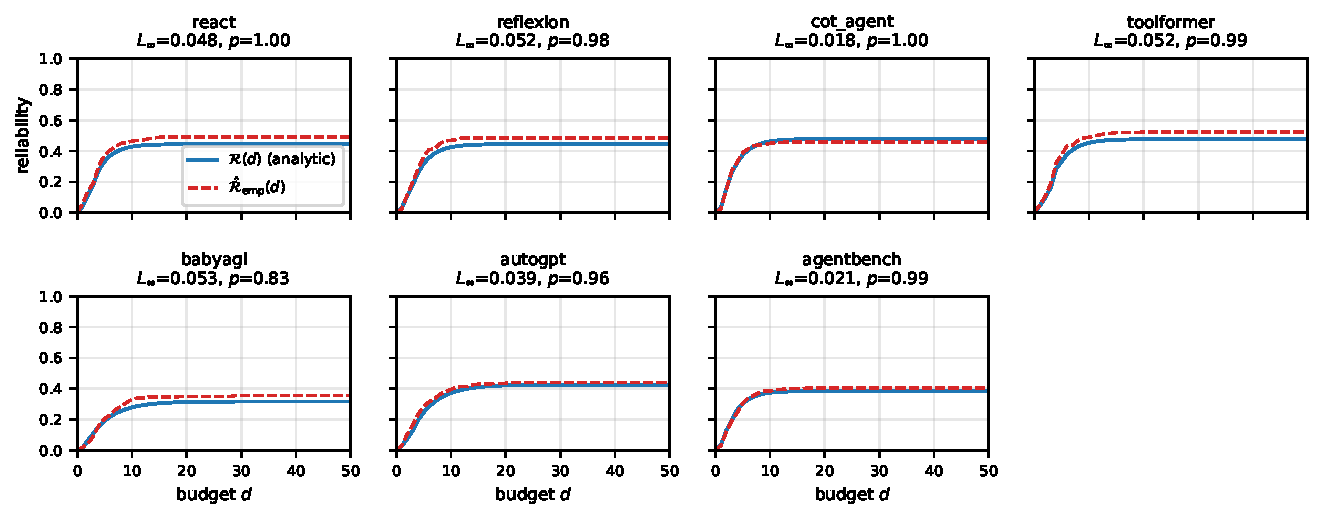
\includegraphics[width=\columnwidth]{../figs/fig_rdc_overlay.pdf}
  \caption{SS9: held-out empirical RDC over the analytic $\mathcal R(d)$.}
  \label{fig:rdc_overlay}
\end{figure}

\paragraph{Findings.}
Figure~\ref{fig:rdc_overlay} overlays, for each framework, the held-out
empirical RDC $\hat{\mathcal R}_{\mathrm{emp}}(d)$ (dashed) on the
analytic $\mathcal R(d)$ of the fitted chain (solid), with each panel
title reporting that framework's $L_\infty^{\mathrm{RDC}}$ and
$p_{\mathrm{KS}}$. The two curves track each other over the whole budget range
$d\in[0,50]$---worst case $0.053$ on babyagi---including the saturation
elbow that the closed form must reproduce to answer horizon queries. Across
all 7 frameworks, the composite diagnostic passes on held-out data at
$\alpha=0.05$. KS distances are small
($D_{\mathrm{KS}}\in[0.020,0.045]$), the minimum KS $p$-value is
$0.827$, and $\max L_\infty^{\mathrm{RDC}}=0.053$ with median $0.048$.
BabyAGI has the largest RDC discrepancy yet still passes KS. This
supports recovery of the success first-passage distribution and RDC
for these controlled MAST-style traces.

\paragraph{Scope.}
SS9 uses synthetic traces from a genuine absorbing chain with noisy
emissions, so the held-out KS test probes controlled recovery by the
trace-to-chain pipeline:
featurization, clustering, Markov-order testing, and MLE. It does not
prove that operational agent traces are Markov; \S\ref{sec:ss10} takes
that step on a real corpus. The MAST release itself lacks the
step-level features required by $\phi$.

%% ----------------------------------------------------------------
%% [REDUCTION] The "Cross-Benchmark Generalization" subsection
%% (synthetic SWE-bench / tau-bench / AgentBench archetypes,
%% Table tab:archetypes and Figure fig:cross_bench) is suppressed
%% from the 12-page body: it was a portability exercise for the
%% vocabulary, and it is now superseded by the *real* SWE-bench
%% (SS10, SS14) and *real* tau-bench (SS15) studies. Retained in
%% source and in the artifact (code/sim/SS7_cross_benchmark.py,
%% figs/fig_cross_benchmark.pdf).
%% ----------------------------------------------------------------
\iffalse
\subsection{Cross-Benchmark Generalization}
\label{sec:cross_benchmark}

Agent evaluation spans diverse environments. To show that the
first-passage vocabulary is not tied to one taxonomy, we construct
synthetic archetypes for three benchmark shapes:
SWE-bench (software engineering)~\cite{swebench2024}, $\tau$-bench
(conversational tool-use)~\cite{taub2024}, and AgentBench
(multi-environment step-based reasoning)~\cite{agentbench2024}.
This is a portability exercise for the vocabulary, not empirical
validation on raw benchmark trajectories; the latter is carried out on
\emph{real} SWE-bench traces in \S\ref{sec:ss10}--\ref{sec:ss14} and on
\emph{real} $\tau$-bench traces in \S\ref{sec:ss15}.

Table~\ref{tab:archetypes} formalizes the mapping from
benchmark-specific behaviors to the Markov state space $\ST$.

\begin{table}[!t]
\centering
\caption{Taxonomy Mapping for Cross-Benchmark Archetypes.}
\label{tab:archetypes}
\begin{tabular}{>{\raggedright\arraybackslash}p{0.22\columnwidth}
                >{\raggedright\arraybackslash}p{0.66\columnwidth}}
\toprule
\textbf{Benchmark} & \textbf{State Taxonomy ($\ST$)} \\
\midrule
SWE-bench~\cite{swebench2024} & \texttt{repo\_setup}, \texttt{issue\_read}, \texttt{search}, \texttt{edit\_file}, \texttt{test\_run} \\
\tstriped
$\tau$-bench~\cite{taub2024} & \texttt{user\_intent}, \texttt{api\_call}, \texttt{api\_resp}, \texttt{user\_clarify}, \texttt{confirm} \\
AgentBench~\cite{agentbench2024} & \texttt{think}, \texttt{act}, \texttt{observe} \\
\bottomrule
\end{tabular}
\end{table}

Using representative transition properties, we compute the same
analytic quantities. Figure~\ref{fig:cross_bench} shows characteristic
RDC behavior across the three archetypes.

\begin{figure}[!t]
  \centering
  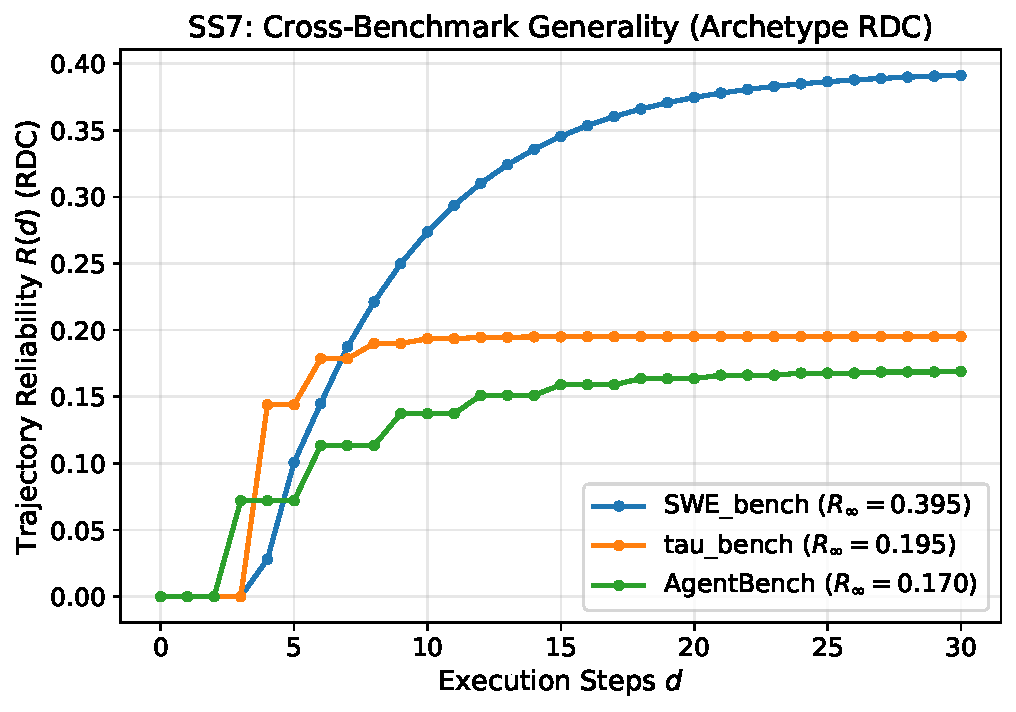
\includegraphics[width=\columnwidth]{../figs/fig_cross_benchmark.pdf}
  \caption{Cross-benchmark archetypes show vocabulary portability:
           RDCs for synthetic state spaces modeling SWE-bench,
           $\tau$-bench, and AgentBench.}
  \label{fig:cross_bench}
\end{figure}

\begin{figure}[!t]
  \centering
  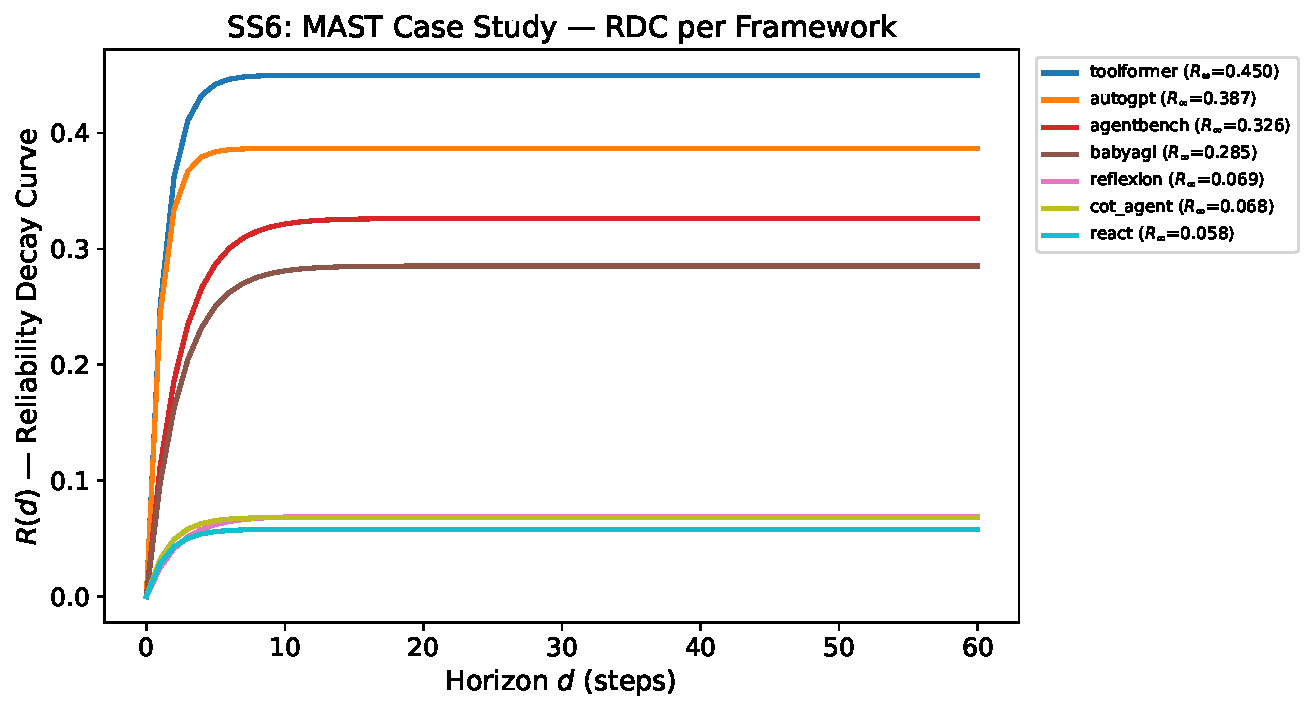
\includegraphics[width=\columnwidth]{../figs/fig_rdc.pdf}
  \caption{SS6 illustrates finite-horizon reliability on MAST-derived
           summaries: reliability decay curves for 7 frameworks ranked
           by $R_\infty$.}
  \label{fig:rdc}
\end{figure}
\fi
%% [END REDUCTION — cross-benchmark archetypes + SS6 RDC figure]

These case studies support a narrow claim: when the diagnostics accept
the trace-to-chain abstraction, the fitted chain provides a coherent
reliability vocabulary for horizons and frameworks, with the limits set
by the available trace representation and the GoF diagnostics.

%% ================================================================
